\documentclass[class=book, crop=false, oneside, 12pt]{standalone}
\usepackage{standalone}
\usepackage{../../style}
\usepackage{../../glossary}
% \usepackage{../../music-tools}
\graphicspath{{./assets/images/}}


% \provideboolean{isCompiledFromMain}
% \setboolean{isCompiledFromMain}{false}


% arara: lualatex
% arara: biber
% arara: latexmk: { clean: partial }
\begin{document}
    \chapter{I Pink Floyd}
    \label{ch:01-pinkfloyd}
    Introdurre i Pink Floyd e contestualizzare la loro carriera e importanza nel panorama discografico non è un'impresa semplice. Protagonisti di un percorso musicale della durata di oltre 45 anni, autori del terzo disco più venduto della musica leggera, innovatori e pionieri di nuove tecniche di registrazione e produzione, i Pink Floyd sono forse il gruppo musicale che più di ogni altro ha saputo catalizzare gli sviluppi della musica pop e rock fino a quel momento e, al contempo, proporre una formula incredibilmente appetibile per un pubblico di massa. In questa trattazione non abbiamo né la pretesa, né tantomeno l'obiettivo a fornire un'analisi completa del gruppo. Piuttosto, intendiamo fornire una concisa ma completa panoramica di alcuni aspetti della loro carriera, in particolare quelli che riteniamo più rilevanti per la trattazione che segue. 

    La trattazione di questo capitolo è articolata come segue. In Sec.\ref{sec:01-bio} riassumeremo in breve la vienda biografica dei Pink Floyd. In Sec.\ref{sec:01-componenti} presenteremo i più importanti componenti della formazione storica. In Sec.\ref{sec:01-musicianship} tracceremo i nodi fondamentali della proposta artistica e musicale dei Pink Floyd. Infine, in Sec.\ref{sec:01-gear} approfondiremo la strumentazione tastieristica impiegata nel corso degli anni da Richard Wright.

    \section{Biografia Essenziale}\label{sec:01-bio}
    \subsection{Nascita e primi anni}
    Il primo nucleo della band che successivamente sarebbe diventata nota con il nome di Pink Floyd si può individuare nei \emph{Sigma 6}, gruppo nato dall'incontro tra Nick Mason e Roger Waters nei corridori della facoltà di architettura della \emph{University of Westminster} a Londra nel 1963. Successivamente noti come \emph{The Tea Seat} e dediti principalmente a cover di brani R\&B, il gruppo era composto da Nick Mason alla batteria, Roger Waters alla chitarra solista, Richard Wright alle tastiere e in qualche occasione alla chitarra ritmica; inizialmente vi facevano parte anche Keith Noble e Clive Metcalfe, che però presto avrebbero lasciato il complesso. Come rimpiazzo, Waters imbracciò il basso e il gruppo ingaggiò Bob Klose alla chitarra solista e Chris Dennis come voce solista; a questi si aggiunse inoltre il chitarrista Syd Barrett, vecchio amico d'infanzia di Waters.
    
    È con questa formazione che il gruppo riesce a fare le prime sedute in studio nel dicembre 1964, ospiti nello studio di registrazione di un amico di Wright. Poco tempo dopo, nel 1965, vennero ingaggiati come resident band per un locale di nome \emph{The Countdown Club}; l'incarico prevedeva che il gruppo suonasse tre set da 90 minuti al giorno. Nello stesso anno, Dennis avrebbe lasciato la band poiché coscritto nella \emph{Royal Air Force}; il suo abbandono sarà presto seguito da quello di Klose, mosso da pressioni da parte dei genitori rispetto alla carriera accademica. Barrett assunse quindi il duplice ruolo di chitarrista e cantante solista e, implicitamente, di leader creativo; si cristallizzò  quindi la prima formazione stabile della band. Evidenza del peso di Barrett nel processo decisionale e creativo è il cambio di nome definitivo del complesso: fu infatti Barrett a coniare \emph{Pink Floyd}, nome costruito accostando i nomi di due dei suoi artisti blues americani preferiti, \emph{Pink Anderson} e \emph{Floyd Council}.
    
    \subsection{L'era Barrett}
    In questo periodo il gruppo acquisisce progressivamente notorietà attraverso una proficua attività live e, sotto la leadership di Barrett, introduce al sostrato R\&B elementi rock e blues. Il loro stile venne in quel periodo identificato sotto l'ombrello del \emph{rock psichedelico}, anche a seguito dell'uso di sostanze allucinogene fatto dalla band, in particolare da Barrett. L'intensa attività live portò il gruppo a essere notato da \emph{Peter Jenner} e \emph{Andrew King}, i quali restarono colpiti dalle performance e dallo stile della band e si offrirono nel ruolo di manager. Questa collaborazione si tradusse in un salto di qualità in frequenza e dimensione negli eventi live dei Pink Floyd, al netto delle perplessità mosse da parte di alcuni esercenti sull'evoluzione della proposta musicale della band. Infatti, alle cover R\&B il gruppo  il gruppo aveva progressivamente affiancato i lavori sperimentali di Barrett, i quali non sempre erano compresi o apprezzati: si pensi chenel 1966, a seguito di un concerto presso il \emph{Catholic youth club}, il titolare si rifiutò di erogare il compenso pattuito perché, a detta sua, la performance "non era musica". {%
    \parfillskip=0pt
    \parskip=0pt
    \par}
    
    Nonostante questo, alla fine del 1966 il gruppo aveva costruito una discreta fanbase e iniziato a suscitare l'interesse delle etichette discografiche, in particolare di \emph{EMI Columbia}, che garantì al gruppo \textsterling 5000 per la produzione e successiva pubblicazione del primo singolo, \emph{Arnold Layne}, nel marzo 1967. Nonostante il contenuto del testo quantomeno bizzarro (il brano parla infatti di un uomo che ruba e indossa abiti e biancheria femminili), il brano ebbe un discreto passaggio radiofonico, tanto da giustificare la produzione di un video promozionale. A giugno uscì un secondo singolo, \emph{See  Emily Playin'}, che riscosse un successo ancora maggiore e solidificò le basi per la produzione del primo LP della band, \acrfull{pgod}, nell'agosto dello stesso anno; il disco fu un successo e fu pubblicato sia sul mercato europeo, sia in quello statunitense. 
    \begin{wrapfigure}{l}{.45\textwidth}
        \centering
        \subimport{assets/figures}{album_timeline.tex}
        \label{fig:album_timeline}
        % \caption{Album in studio.}
    \end{wrapfigure}
    
    In questo periodo l'uso di allucinogeni da parte di Barrett si intensificò e il resto del gruppo iniziò a osservare spiacevoli episodi di dissociazione da parte già durante la produzione del disco. Questi divvennero più frequenti durante il tour promozionale, e costrinsero il gruppo ad eliminare le date negli Stati Uniti a causa del deterioramento della stabilità mentale di Barrett, che andava spesso incontro a esaurimenti nervosi e crisi di panico. Inoltre, nei concerti effettuati, Barrett eraspesso assente, dava spesso le spalle al pubblico e in qualche caso affossò l'intera performance rifiutandosi di cantare e suonando una sola nota o un solo accordo per l'intera durata dell'evento. Per questi motivi il gruppo introdusse nella band \emph{David Gilmour}, un vecchio amico di Barrett. 
    
    Inizialmente Gilmour avrebbe dovuto suonare live con la band qualora Barrett fosse indisposto, ma ben presto le condizioni di salute di Barrett peggiorarono al punto che era evidente che soffrisse di depressione e forse schizofrenia. Aveva smesso di partecipare alle sedute di registrazione, non parlava con nessuno degli altri membri della band e il suo contributo alla scrittura dei pezzi si ridusse al punto che, nel secondo LP \acrfull{sos} (giugno 1968), un solo pezzo di Barrett era presente: \emph{Jugband Blues}, un brano tanto particolare quanto efficace nell'esprimere il misterioso e contorto stato interiore di Barrett e all'interno del quale emerge la consapevolezza che l'esperienza nell'industria musicale stava per volgere al termine.
    
    Barrett infatto fu estromesso dalla band nell'aprile del 1968 e si ritirò a vita privata, rifuggendo ogni forma di apparizione pubblica e vivendo il resto della sua vita nell'anonimato. Questa scelta con ogni probabilità contribuì a cementificare lo status di mistero e dannazione che avvolge la figura di Barrett, sia di fronte al grande pubblico, ma anche nei confronti dei suoi ex colleghi.
    
    
    \subsection{L'era Waters}
    Al netto degli inconvenienti causati da Barrett, la produzione e il rilascio di \acrshort{sos} ottennero buoni risultati e il disco riuscì a posizionarsi nella nona posizione nelle \emph{UK Charts}. Questo successo promosse un tour transcontinentale in Europa e negli Stati Uniti e la produzione dei due dischi successivi: \acrlong{more} (giugno 1969), colonna sonora del film omonimo, e \acrlong{ug} (novembre 1969). Quest'ultimo segnò un notevole stacco dai precedenti lavori, in termini di ambizione e sperimentazione: si trattava infatti di un doppio album, la cui prima metà era costituita da delle registrazioni live, mentre la seconda metà da materiale inedito e dal carattere fortemente sperimentale. Nonostante la tiepida accoglienza della critica, il gruppo successivamente avrebbe espresso un certo disprezzo nei confronti del disco. Anche il successivo LP  \acrfull{ahm} (ottobre 1970) ebbe un destino simile: fu infatti il primo lavoro nel quale la band collaborò estesamente con altri musicisti (il compositore \emph{Ron Geesin} e il direttore d'orchestra \emph{John Alldis}), nonché il primo disco del gruppo a raggiungere la prima posizione delle \emph{UK Charts}, ma Gilmour e Waters si sarebbero sempre mostrati critici del lavoro.


    Il successivo LP, \acrlong{med} (ottobre 1971), segna un passo importante nella carriera dei Pink Floyd per due motivi: in primo luogo, è il primo disco in cui l'elemento sperimentale e \emph{progressive} diventa trainante e preponderante nel suono e nel marketing della band, perdendo ormai del tutto l'eredità psichedelica dell'era Barrett; in secondo luogo, è qui che la leadership di Waters in termini di testi e scrittura inizia a consolidarsi, nonostante a questo punto il contributo degli altri membri sia ancora importante, in particolare quello di Gilmour. Il successivo disco \acrfull{obc} (1972), conferma queste tendenze.

    Obscured by Clouds fu però quasi subito oscurato dal suo successore. La band tornò agli \emph{Abbey Roads Studios} nel maggio del 1972 e iniziò, con l'assistenza dell'ingegnere \emph{Alan Parsons}, a lavorare a delle demo che Waters aveva realizzato in un piccolo studio allestito nella sua capanna degli attrezzi; tutti i testi furono scritti dallo stesso Waters, e componevano un concept album i cui argomenti includevano avidità, conflitto, morte e salute mentale. Le 10 tracce del disco erano pensate per essere riprodotte senza soluzione di continuità, in linea con la concezione organica tipica dei concept album del progressive di quegli anni. Inoltre, il gruppo fece un uso ampio e creativo di sintetizzatori, campionatori, strumentazione ed effettistica, portando al grande pubblico dei suoni del tutto nuovi. Per tutti questi motivi \acrfull{dsom}, rilasciato nel marzo 1973, può essere considerato il primo disco compiutamente progressive dei Pink Floyd; nonostante questo, fu fin da subito il loro maggior successo commerciale, raggiungendo la prima posizione della \emph{Billboard 200 albums} e rimanendo nella classifica per 736 settimane; vendette 46 milioni di copie, risultando \emph{de facto} il terzo disco più venduto nella storia dell'industria discografica.

    Il gruppo mantenne gran parte degli elementi progressive anche nel successivo \acrfull{wywh} (1975), nel quale i testi di Waters approfondivano il tema dell'alienazione, sia dal punto di vista delle relazioni, sia dal punto di vista dell'industria discografica. Waters trovò grande ispirazione in questo senso nella figura di Barrett e nel suo decadimento. Un episodio notevole avviene il 5 giugno 1975, quando Barrett si presentò in studio senza preavviso. A quel punto, Barrett era diventato calvo, le sopracciglia rasate e leggermente sovrappeso. Inizialmente nessuno lo riconobbe; dopo aver realizzato la sua identità, alcuni membri della squadra scoppiarono in lacrime. Il gruppo a quel punto suonò \emph{Shine on You Crazy Diamond}, ma pare che Barrett non fosse sufficientemente lucido da capire che il pezzo era dedicato a lui.

    Il successivo \acrlong{anm} (1977) da un lato continua il ramo dei concept album, questa volta proponendo una critica alla condizione politico-sociale della società inglese degli anni '70 traendo profonda ispirazione dal romanzo di Orwell \emph{Animals Farm}; dall'altro, segna la formazione di una prima crepa nella formazione. Waters stava infatti assumendo un controllo sempre più profondo sulla scrittura e la direzione musicale dei Pink Floyd, e questo causava delle discussioni di carattere sia personale, sia pecuniario. 
    
    Il tour promozionale di Animals fu inoltre segnato da alcuni incidenti con alcuni spettatori degli eventi live: ad esempio, a seguito di un concerto a Montreal, Waters sputò in viso a un fan che lo aveva raggiunto per dirsi insoddisfatto della performance di quella sera. Questi episodi ispirarono Waters nella scrittura del successivo \acrfull{tw} (1979), un doppio concept album su alienazione, abbandono e solitudine vista attraverso gli occhi di \emph{Pink}, una fittizia rockstar depressa in preda a delle riflessioni profonde sulla propria carriera. Rilasciato in fretta a causa di incombenti difficoltà economiche, il disco si rivelò fortunatamente un successo, vendendo più di 30 milioni di copie; vennero estratti tre singoli (\emph{Another Brick in the Wall, Part 2}, \emph{Run Like Hell} e \emph{Comfortably Numb}) e tutti e tre diventarono hit radiofoniche. 
    
    La produzione di \acrshort{tw} vide anche l'estromissione dalla band di Wright, il quale stava attraversando alcuni problemi personali che gli impedivano di dare qualsivoglia tipo di contributo alla produzione del disco; nonostante questo, partecipò lo stesso al tour in qualità di session man stipendiato. Conseguentemente, Wright non partecipò nemmeno alla produzione del successivo \acrfull{fc} (1983). Il disco ricevette un'accoglienza tiepida e fu il disco meno venduto dai tempi di Obsucred by Clouds; questo, assieme a tanti altri motivi di carattere personale e musicale, alimentò il crescente conflitto tra Waters e Gilmour. Queste tensioni sfociarono nell'abbandono della band da parte di Waters, convinto che il gruppo non avesse più alcun futuro. Gilmour invece, una volta vinta la diatriba legale con Waters per il controllo del nome, decise assieme a Mason di reintrodurre Wright e portare avanti l'esperienza dei Pink Floyd.

    \subsection{L'era Gilmour}
    Assieme al produttore Bob Ezrin, che già aveva collaborato con il gruppo per la produzione di The Wall, la band mise assieme del materiale che confluì in \acrfull{mlor} (1987), disco che ottenne un discreto successo e dal quale furono estratti tre singoli che ebbero un considerevole passaggio radiofonico (tra i quali \emph{Learning to Fly}). In seguito al tour promozionale, le attività a nome dei Pink Floyd vennero messe in pausa  e i tre membri del gruppo perseguirono ciascuno delle proprie attività da solista. Nel 1993 i tre si trovarono in studio assieme a Bob Ezrin per registrare nuovo materiale, in gran parte preparato da Gilmour e Wright. Il risultato fu \acrfull{db} (1994), seguito anch'esso da un imponente tour promozionale. In seguito, le attività della band si fermarono per circa vent'anni.

    Nel 1997 il gruppo fu invitato a Los Angeles per essere introdotto nella \emph{Rock And Roll Hall of Fame}, ma solamente Gilmour, Wright e Mason si presentarono; Barrett non rispose alla chiamata, e Waters rifiutò ogni sorta di coinvolgimento. Nove anni dopo, in occasione del \emph{Live Aid} a \emph{Hyde Park}, avvenne il tanto agognato ricongungimento di Waters con il resto della band; il concerto fu un successo enorme, ma non fu seguito da alcun tipo di ripresa delle attività in studio o live. Tuttavia, nel 2007 il gruppo organizzò un grande concerto in memoria di Barrett, morto l'anno prima di cancro al pancreas.

    L'anno successivo, nel 2008, Wright morì di un tumore ai polmoni. Questo evento fu motivatore per il ritorno in studio di Gilmour e Mason, i quali recuperarono parte del materiale scartato durante la produzione di The Division Bell e lo completarono, rilasciando quindi, nel 2014, \acrfull{er}, quindicesimo e ultimo album dei Pink Floyd.

    \section{Componenti}\label{sec:01-componenti}
    \paragraph{Syd Barrett}
    Chitarrista, cantante e principale compositore e paroliere fino al 1968. Nonostante il carattere fortemente improvvisato della musica psichedelica, Barrett è stato un chitarrista a suo modo innovativo: ha esplorato l'uso del delay e tentato l'uso del feedback a fini creativi. Tra i suoi suoni più famosi si annovera quello ottenuto processando il segnale della chitarra con una echo box e facendo scivolare un accendino zippo lungo le corde. 
    \paragraph{Roger Waters}
    Bassista, cantante e principale compositore e paroliere fino al 1983. Come la maggior parte dei bassisti degli anni '60, era nato originariamente come chitarrista; vestigia di questo passato si può notare nell'uso frequente di riff come ossatura per le basslines e per il songwriting (\emph{Money}). Le sue linee melodiche erano essenziali sia in quanto a pattern ritmici (coerentemente allo stile di Mason), sia in quanto a scelte melodiche, in modo da lasciare ampio spazio all'arrngiamento e alle chitarre. Waters era solito usare il basso in maniera piuttosto creativa: ad esempio, i pattern ritmici di \emph{Time}, \emph{Obscured by Clouds} e \emph{Childhood's End} sono stati tutti creati da Waters mutando le corde e prestando grande attenzione all'articolazione delle pennate.
    \paragraph{Nick Mason}
    Batterista formatosi principalmente nel jazz e nel mondo dell big bands. Contrariamente alla maggior parte dei batteristi rock dell'epoca, in studio era solito proporre arrangiamenti delicati e seduti, prediligendo fill semplici e pattern ritmici essenziali; tuttavia, durante i concerti, in supporto alla grande dinamicità dei live dei Floyd, era capace di alzare molto la dinamica e sorreggere la maestosa impalcatura ritmica e scenica degli eventi.
    \paragraph{Richard Wright}
    Tastierista e cantante. Wright era un prolifico polistrumentista di formazione sia classica, sia jazz. Quest'ultimo genere costituisce la sua principale influenza nella produzione dei Pink Floyd: Wright era principalmente un improvvisatore, raramente preparava strutture e partizioni accurate per le parti che doveva suonare; pare che questa insofferenza verso le parti scritte fu una delle cause delle tensioni covate durante la produzione di The Wall, disco dagli arrangiamenti rigidamente scritti. Le sue influenze principali erano Miles Davis e John Coltrane; l'uso di accordi e soluzioni direttamente ispirati da questi ultimi era frequente (si pensi al passaggio D\(^{7 \sharp 9}\) - D\(^\textrm{o}\) in \emph{Breathe}, direttamente ispirato da \emph{A Kind of Blue}). 
    \paragraph{David Gilmour}
    Chitarrista e cantante, in seguito principale compositore e paroliere a partire dal 1983. Come tutti gli altri membri, Gilmour era un chitarrista lontano dal virtuosismo e più attento al tocco e alle trame armoniche. Le sue parti erano caratterizzate da idee melodiche semplici ma di grande impatto, un fraseggio distintamente blues dato dall'uso di scale pentatoniche, bending (spesso anche di tono e mezzo) e un caratteristico vibrato. L'assenza di una ricerca spasmodica del virtuosismo non impedì a Gilmour di produrre assoli di notevole impatto e durata: come esempi, impossibile non citare quelli di \emph{Time}, \emph{Money}, \emph{Dogs} e \emph{Comfortably Numb}.

    \begin{figure}[H]
        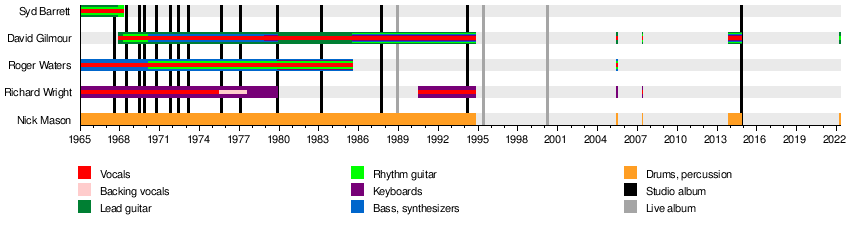
\includegraphics[keepaspectratio, width=\textwidth]{pinkfloyd-timeline.png}
        \label{fig:01-pinkfloyd-timeline}
        \caption{Cambiamenti di formazione nei Pink Floyd}
    \end{figure}
    
    \section{Profilo musicale}\label{sec:01-musicianship}
    
    \subsection{Genere}
    Accostare la musica dei Pink Floyd nel suo complesso a un particolare genere è un'operazione piena di insidie e destinata a risultare in un'analisi fragile nel migliore dei casi, o del tutto errata nel peggiore. Questo perché la direzione musicale dei Floyd non è monolitica, bensì è meglio rappresentabile come un \emph{continuum} evolutivo della durata di oltre 25 anni; per comodità consultativa e in analogia alla trattazione biografica (\ref{sec:01-bio}), possiamo ripartire la discussione secondo le tre leadership che si sono succedute nell'arco di vita del gruppo.

    \paragraph{Psichedelica - Barrett}
    I Floyd di Barrett sono stati dei pionieri della \emph{psichedelica}, uno stile dei tardi anni '60 sviluppatosi parallelamente sia nella scena underground londinese (di cui gli stessi Floyd facevano parte), sia nella scena statunitense (\emph{The Doors}, \emph{Jefferson Airplane}). La psichedelica non aveva dei tratti propriamente musicali che la contraddistinguessero da altri stile dell'epoca. Di fatto, i tratti comuni di questi gruppi era la predilizione per una scrittura di lunghe composizioni, simili a delle \emph{suite} ma molto meno rigide e costituite da poche sezioni dalle trame armoniche semplici e lunghi passaggi improvvisati, spesso ispirati dall'uso sistematico e "ideologico" di sostanze psicotrope e allucinogene (in particolare LSD); in questo canovaccio trovavano posto molti degli stili più in voga all'epoca (hard rock, blues, folk, country). Esempio paradigmatico di questo stile possono \emph{Interstellar Overdrive} o \emph{Astronomy Dominé}, entrambe da \acrshort{pgod} (1968); esempi d'oltreoceano possono essere \emph{Light My Fire} (\emph{The Doors}) e \emph{In a Gadda Da Vida} (\emph{Iron Butterfly}).

    \paragraph{Progressive - Waters}
    Durante il periodo Waters, il più lungo, denso e prolifico per la band, il genere dei Pink Floyd viene solitamente accostato al \emph{progressive rock} e quindi associato alla scena inglese e internazionale degli anni '70, assieme a gruppi come \emph{Genesis}, \emph{Yes}, \emph{ELP}, \emph{Kansas}, \emph{PFM} e \emph{Banco del mutuo soccorso}. La musica prog si proponeva di elevare il carattere popolare della musica pop e rock al tempio della musica colta; le canzoni prog erano spesso lunghe suite articolate, con frequenti cambi di tempo, bpm e tonalità; le progressioni armoniche erano complesse e mutuate dalla musica colta, frequentissimo l'uso di tempi dispari, ostinati, pedali, le trame e gli arrangiamenti erano ricercati, il virtuosismo incentivato e l'interesse per le nuove tecnologie di sintesi sonora e campionamento era intenso. Gli album erano composizioni omogenee dal punto di vista lirico e compositivo (\emph{concept album}), e spesso le varie tracce si succedevano senza soluzione di continuità.

    All'interno di questo panorama, i Pink Floyd rappresentano un caso singolare. Seppero infatti abbracciare molti dei tratti del genere: i testi erano profondi e impegnati e spesso ascritti a dei concept album (spesso anche omogenei dal punto di vista armonico: Dark Side fa ampio uso del dorico, in The Wall l'uso delle none costituisce un \emph{fil rouge}), frequenti le lunghe suite dalle trame armoniche e arrangiamenti ricercati; le sperimentazioni sonore e l'uso dei sintetizzatori forse l'elemento esplorato dai Floyd più che da chiunque altro. Tuttavia, il virtuosismo era molto ridotto, così come l'uso dei tempi dispari (\emph{Money} eccezione notevole in tal senso); inoltre, le radici blues e folk furono mantenute e incorporate nel nuovo stile (frequente l'uso di strutture mutuate dal blues, come ancora \emph{Money}, o della chitarra acustica negli arrangiamenti). Tutto questo rese i Floyd il gruppo prog dal maggior successo commerciale dell'epoca e, contemporaneamente, il gruppo la cui fama e influenza si dimostrò più resiliente al trascorrere del tempo.

    \paragraph{Ambient - Gilmour}
    Di fatto, dovendo cercare un'etichetta per il genere musicale dei Floyd dell'era Gilmour, la più appropriata rimarrebbe comunque quella di progressive rock. La maggior parte degli elementi era rimasta anche in Momentary Lapse e Division Bell: concept omogeneo, sperimentazione sonora (anche se non più d'avanguardia come negli anni '70), scrittura e armonie non convenzionali. 

    È però impossibile non riconoscere la personale impronta stilistica data da Gilmour in questo periodo: le soluzioni armoniche erano meno jazzistiche e più "aperte", gli arrangiamenti più ampi, spaziosi, così come le idee melodiche sviluppate, in piena coerenza con la scrittura che Gilmour aveva sempre avuto. I sintetizzatori non erano più protagonisti, bensì usati per creare densi ma delicati tappeti sonori. Tutti questi tratti cospargono gli ultimi lavori dei Pink Floyd, in particolare Division Bell, di una sottile patina \emph{ambient}, particolarmente evidente in brani come \emph{Marooned} e \emph{High Hopes}.

    \subsection{Testi}
    L'immagine dei Pink Floyd è indissolubilmente legata alla produzione lirica cupa e disillusa di Waters. Nonostante inizialmente la scrittura dei testi fosse riprartita in maniera bilanciata tra i vari membri, Waters ne assunse man mano un controllo sempre maggiore, al punto da scrivere da solo la totalità dei testi  di Animals e The Wall. I testi di Waters toccavano temi come l'alienazione nella società e nell'industria discografica, l'avidità e le aspettative di vita, le ripercussioni della moderna concezione del tempo nella salute mentale degli individui, l'autorealizzazione, la guerra, lo sfruttamento e l'oppressione verso le masse perpetrata dal potere costituito. 

    La determinazione di Waters nell'esprimere i suoi cupi umori interni erani tali che, in occasione di The Wall, scrisse una sceneggiatura che, in una cinquantina di pagine, riprendeva ed estendeva la storia di Pink, il fittizio protagonista di The Wall; questa fu in seguito ampliata e finalizzata alla realizzazione di una produzione cinematografica vera e propria: il film \emph{Pink Floyd - The Wall}, diretto da \emph{Alan Parker} e prodotto da \emph{Metro-Goldwyn-Mayer}, fu rilasciato nel luglio 1982.

    \subsection{Eventi live}
    I Pink Floyd dedicarono la massima cura e importanza nella preparazione degli eventi live. Furono pionieri dell'utilizzo di luci, laser ed effetti visivi nel palco in funzione dell'evento stesso; durante queste esibizioni, molto spesso gli stesi musicisti arretravano o uscivano dal palco, lasciando quindi i giochi di luce protagonisti. Le novità sonore non furono da meno: si pensi ad esempio all'uso dell'Azimoth co-ordinator, un sistema di gestione di quadrifonia manovrato in tempo reale da Wright e del cui uso furono pionieri.

    Nel corso degli anni '70 i live si fecero via via più spettacolari. Nel 1973 fu introdotto il caratteristico schermo circolare dietro al palco, da lì in poi presenza fissa negli eventi; nel tour di Animals furono realizzati dei giganteschi pupazzi di cani maiali e pecore; per ogni live del tour di The Wall veniva realizzato un muro di cartapesta alto dodici metri a separare musicisti e pubblico, sopra al quale scorrevano delle sequenze animate, e che crollava sul finale.



    \section{La strumentazione di Richard Wright}\label{sec:01-gear}
    Le sperimentazioni a livello sonoro sono uno degli elementi più distintivi e riconoscibili dell'estetica musicale dei Pink Floyd; il gruppo si è sempre premurato di restare aggiornato sui più recenti sviluppi dell'industria di sintetizzatori e campionatori, e il loro uso è sempre stato un elemento importante, tanto da cotituire quasi interamente la ragion d'essere e il fine compositivo di alcuni brani. Per questi motivi è importante proporre un'analisi non superficiale della strumentazione che, nel corso degli anni, è stata acquistata e impiegata dai Floyd.

    L'analisi riproposta in questa sezione si concentra sugli strumenti impiegati da Wright e comprende sia gli strumenti acustici e classici, sia il vasto repertorio di sintetizzatori. Le informazioni riportate sono extrapolate dall'ottima analisi presentata in \cite{azimuth2004gear} e integrate qualora opportuno.
    
    \subsection{Pianoforti acustici}
    L'utilizzo del pianoforte acustico, benché non preponderante, ha caratterizzato il suono dei Pink Floyd fin dai primi dischi. A differenza della prassi dell'epoca, Wright ha sempre preferito utilizzare pianoforti acustici anche durante i tour degli anni '70, quando invece per molti altri artisti era prevalente la tendenza a sostituire ogni parte di pianoforte acustico con dei più pratici pianoforti elettrici; chiaro esemprio è dato dal tastierista dei Genesis Tony Banks, che sul palco utilizzava un pianoforte elettrico per suonare anche un brano dal suono iconicamente acustico come l'intro di \emph{Firth of Fifth}. 
    
    Diventa naturalmente difficile dire quale marchio o modello di pianoforte acustico sia stato usato durante le registrazioni degli LP; tuttavia, da quanto emerge da interviste e documentari, \emph{Steinway \& Sons} e \emph{Yamaha} sembrano essere i marchi preferiti da Wright. Ad esempio, uno \emph{Steinway \& Sons Baby Grand Piano} è usato durante la produzione di Dark Side agli Abbey Road, come si può vedere in alcuni documentari. Uno \emph{Yamaha C7} dovrebbe invece essere stato usato durante alcuni dei primi album e di nuovo in Animals e The Wall.

    A partire dal 1987, i pianoforti furono sostituiti in live dai campioni del \emph{Kurzweil K2000}; questa serie di workstation fu utilizzata anche durante la produzione di The Division Bell, limitatamente alla produzione di demo.

    \subsection{Pianoforti elettrici}

    \paragraph{Wurlitzer EP}
    Il suono dei pianoforti elettrici Wurlitzer divenne presto uno dei tratti distintivi del suono dei Pink Floyd degli anni '70. Wright fece uso soprattutto della serie \emph{EP-200}, contraddistinta da un attacco più pronunciato, che ricordava il suono di un vibrafono, e un sustain e tremolo più delicati, rendendone rendendo il suono più virante al funky rispetto all'equivalente Rhodes. Il Wurly fu impiegato per la prima volta in Obscured by Clouds e, in seguito, più estesamente in Dark Side e Wish You Were Here. Esempi notevoli sono \emph{Breathe}, \emph{Time}, \emph{Have a Cigar}; in \emph{Shine On You Crazy Diamond, Part 8} viene utilizzato in funzione solistica, mentre in \emph{Money} viene utilizzato in accoppiata con un \emph{Cry Baby wah-wah pedal} durante la sezione centrale di assoli. 

    \paragraph{Fender Rhodes Stage/Suitcase EP}
    La serie EP di Rhodes (successivamente acquisita da Fender), in particolare il Mark I, era caratterizzata da un timbro più jazzistico e più adatto alla realizzazione di passaggi melodici e soli rispetto al Wurly, impiegato prevalentemente in accompagnamenti ritmici. Wright già possedeva un \emph{Rhodes Suitcase Mark I} all'inizio degli anni '70, usato ad esempio in \emph{Mudman} di Obscured by Clouds; temporaneamente abbandonato in favore del Wurly, il Mark I venne rispocerto e riutilizzato specialmente in Animals (intro di \emph{Sheep}) e The Wall (\emph{Hey You}). Come da prassi negli anni '70, il Mark I non veniva utilizzato in line-in nel mixer, ma era collegato a un amplificatore, il quale veniva poi ripreso come fosse una chitarra; la scelta di Wright cadeva solitamente sul \emph{Fender Twin Reverb}.

    Come accadde anche per i pianoforti acustici, a partire dal 1987 anche i pianoforti elettrici furono sostituiti dalle più moderne workstation campionatori; in quegli anni, la scelta era sempre il K2000, utilizzato da Wright anche per lel registrazioni del suo disco solista \emph{Broken China} (1996).

    \paragraph{Hohner Clavinet}
    Il clavinet è uno strumento a tastiera caratterizzato da un attacco estremamente pronunciato e un veloce decay; questa configurazione d'inviluppo conferisce al timbro staccati molto efficaci e, per questo, lo strumento viene ampiamente utilizzato in funzione ritmica nel genere funky (\emph{Superstition} di \emph{Stevie Wonder} è di certo il miglior esempio in tal senso). Nonostante non fosse mai la prima scelta per Wright, preferendo il timbro più rotondo e meno aggressivo del Wurly negli accompagnamenti ritmici, egli possedeva uno \emph{Hohner D6}, che venne impiegato nell'arrangiamento di \emph{Have a Cigar} e \emph{Shine On You Crazy Diamon, Part 8} (circa minuto 7:00). Viene utilizzato anche in \emph{Pigs (Three Different Ones)}, anche se è molto nascosto nel mix. Viene sporadicamente impiegato anche in \emph{Wet Dreams} (1978), il primo album solista di Wright.

    \paragraph{Yamaha CP-70 EP}
    Il \emph{CP-70} completa il trio dei più iconici suoni di pianoforte elettrico degli anni '70. A differenza del Wurly e del Rhodes, il CP-70 trovò un impiego piuttosto limitato nell'estetica musicale dei Pink Floyd. L'unica occasione in cui ne fecero uso rilevante fu durante ill tour di The Wall, dove venne usato dallo session man Pete Woods, che affiancava Wright per il tour, per sostituire alcune parti di Rhodes.

    \subsection{Organi}
    \paragraph{Organi Farfisa}
    Nei primi anni dei Pink Floyd, i Farfisa sono stati la prima scelta di Wright per quanto riguarda i suoni di organo. Si trattava di un organo compatto a due manuali, come la maggior parte dei modelli di Hammond, ma era caratterizzato da un suono meno aggressivo. Wright aggiunse alla sua unità Farfisa anche un \emph{Binson Echoreic}, un modulo che produceva effetti di modulazione temporale al suono e che Wright riuscì a sfruttare sapientemente per creare suoni mobili e interessanti, costituendo uno dei primi tentativi di sperimentazione sonica dei Pink Floyd e udibile già a partire da \acrshort{pgod}. Come detto, il Farfisa fu lo strumento principale di Wright ed era usato sia in studio che live; per riprodurre gli effetti di modulazione basati sul pan nei soli in live, Wright si servì di un dispositivo (\emph{azimuth co-ordinator pot}).

    Verso la fine degli anni '60 il Farfisa sparì dalla dotazione live di Wright, ma restò negli studi fino alla produzione di Dark Side; l'ultima traccia ad includere il Farfisa fu infatti l'intro di \emph{Time}.

    \paragraph{Organi Hammond}
    Al Farfisa Wright ha presto introdotto degli organi prodotti da Hammond, che negli anni '70 stavano rapidamente crescendo in popolarità. Erano prodotti in accoppiata con dei cabinet \emph{Leslie}, che era dotato di un componente rotante. Questo elemento era nato inizialmente per rimuovere la percussione nell'attacco del suono dell'organo, considerata poco desiderabile nell'estetica della musica ecclesiastica per cui era originariamente pensato; il risultato fu che il Leslie conferì all'Hammond un distintivo effetto tremolo che contribuì a far emergere in quanto a qualità e versatilità il timbro di Hammond fra i vari concorrenti, come il Farfisa.

    Wright utilizzò svariati modelli di Hammond: iniziò con un \emph{M102} (modello a spinetta) acquistato nel 1968, per poi sostituirlo con un \emph{RT3} a due manuali e approdando infine sui più popolari \emph{B3} e \emph{C3}, a seconda dello studio di registrazione in cui si trovava.
    
    \subsection{Sintetizzatori e campionatori}
    \paragraph{Mellotron}
    Il Mellotron è uno dei primi tentativi di ingegnerizzazione di uno strumento in grado di riprodurre campioni. Si trattava di uno strumento a tastiera i cui tasti, premuti, attivavano la riproduzione di dei nastri magnetici su cui erano incisi i suoni di svariati strumenti a fiato e ad arco. Visto come un campionatore, era uno strumento piuttosto limitato: la qualità delle registrazioni su nastro era scadente, lo strumento era fragile a causa della natura dei supporti di registrazione e, trattandosi di registrazioni, la durata di ogni nota era limitata a circa 7 secondi.

    L'utilizzo del Mellotron da parte di Wright fu molto sporadico: nonostante fosse utilizzato piuttosto trasversalmente da altri gruppi del periodo (Beatles, Led Zeppelin, Genesis), il Mellotron non fece mai parte dell'equipaggiamento live dei Pink Floyd. Atom Heart Mother e \acrshort{ug} furono i dischi in cui il suo uso è più notevole, soprattutto nelle rispettive suite (\emph{Atom Heart Mother} e \emph{Sysyphus}). Wright preferiva condire i suoni prodotti con riverberi e altri effetti di modulazione temporale, mascherando il timbro tipico dei suoni del Mellotron, che risulta quindi meno apparente dell'equivalente dei dischi di altri gruppi dell'epoca.

    \paragraph{EMS VCS3, Synthi A, KS}
    L'\emph{Electronic Music Studios Voltage Controlled System model 3} voleva essere una risposta britannica ai prodotti dell'americana \emph{Moog}. Il VCS3 era un synth portatile con 3 VCO (voltage controlled oscillators), un noise generator, un ring modulator e altri moduli. Gli oscillatori erano capaci di produrre sinusoidi, square waves e sawtooth waves, che potevano essere processate attraverso un ring modulator e un assortimento di filtri. EMS produsse anche una versione suitcase del VCS3, il \emph{Synthi A}; quest'ultima fu impiegata in Meddle, in particolare in \emph{One of These Days} e \emph{Echoes}. Fu però la successiva revisione, il \emph{Synthi A KS}, a essere esplorata dalla band: alle specifiche del Synthi A aggiungeva una tastiera blu piatta e touch-sensitive e un sequencer, il cui uso si può già sentire in \emph{Free Four} di Obscured by Clouds. Il KS fu poi impiegato per le sequenze di \emph{On the Run} e \emph{Time}. Fu poi impiegato sui successivi Wish You Were Here (\emph{Welcome to the Machine} e negli sweep simil-vento di \emph{Shine On You Crazy Diamond}). Spesso si dice che il VCS3 fu usato per creare i pattern ritmici di \emph{Obscured by Clouds}, \emph{Childhood's End} e \emph{Time}; in realtà, quegli effetti erano stati prodotti da Waters con il suo P-bass.

    \paragraph{Minimoog}
    Il \emph{Minimoog} è forse uno dei marchi più riconoscibili del suono del rock degli anni '70, data la sua trasversale diffusione nell'ambiente prog. A partire da Dark Side, il Minimoog fu il sintetizzatore preferito per la creazione dei lead, in opposizione ai synth di famiglia VCS3, utilizzati soprattutto per creare effetti d'ambiente. Alcuni esempi notevoli di lead sono \emph{Any Colour You Like}, il lead simil-ottone in \emph{Shine On You Crazy Diamond} e il riff principale di \emph{Have a Cigar}. Sempre in Diamond, Wright utilizzò anche il \emph{Moog Taurus II Footpedal}, una sorta di Minimoog depotenziato  e azionato tramite una tastiera a pedali. A partire dalla produzione di The Wall, il Minimoog iniziò a essere sostituito dai sintetizzatori polifonici: ad esempio, il solo di \emph{Run Like Hell} suona simile a un Minimoog, ma con ogni probabilità si tratta di un \emph{Prophet V}.

    \paragraph{ARP Solina String Ensamble}
    ARP era un marchio americano che produceva sintetizzatori noti per come riproducevano gli strumenti ad arco; un \emph{Solina String Ensamble} venne utilizzato in studio già dal 1972, in \emph{Childhood's End} e \emph{Absolutely Curtains} di Obscured by Clouds. Successivamente, a partire dal 1974, Wright introdusse un \emph{Solina model V} nel suo equipaggiamento e lo sfruttò più intensamente in \emph{Shine On You Crazy Diamond}, in tutto Animals e nel tour di The Wall.

    \paragraph{Yamaha GX1}
    Lo \emph{Yamaha GX1} è una sorta di chimera nel mondo dei sintetizzatori: estremamente raro, complicato da programmare, tanto fragile quanto estremamente versatile in quanto a timbri riproducibili grazie alle sue tre tastiere, molteplici modalità di interfacciarsi a esse, filtri ed effetti più disparati. John Paul Jones ne aveva uno, Stevie Wonder e Keith Emerson ne avevano due; è noto e documentato che Wright ne abbia posseduto uno, probabilmente per un breve periodo di tempo; non è chiaro quando di preciso lo abbia posseduto, ma è certo che non fu mai utilizzato in alcuna registrazione da aprte sua, né per i Pink  Floyd, né nei suoi progetti solisti.

    \paragraph{SCI Prophet V}
    Il \emph{Prophet V} era un sinstetizzatore analogico polifonico dalla versatilità senza uguali per l'epoca. Era completamente programmabile e aveva un vasto assortimento di suoni, effetti, filtri, modulatori d'inviluppo e LFO. Per questi motivi, diventò presto il sintetizzatore più diffuso dei primi anni '80, usato da \emph{Peter Gabriel}, \emph{Rick Wakeman}, \emph{Vangelis} e \emph{Richard Barbieri} (il quale ha continuato fino a pochi anni fa a tenerlo come sintetizzatore principale nel suo eguipaggiamento). Anche Wright se ne procurò uno nel 1978, in sostituzione di un meno versatile \emph{Oberheim 4-voices Polyphonic}; tuttavia, a causa dei problemi che stava attraversando in quel periodo sia a livello privato, sia con gli altri membri della band e in particolare Waters, non furono molte le parti di sintetizzatore suonate da Wright che furono incluse nel disco finale (questo fu anche dovuto alla diversa genesi, natura e composizione di The Wall rispetto ai precedenti). Tuttavia, eccezione notevole di è rappresentata da \emph{Run Like Hell}, che include un assolo di synth suonato da Wright con il suo Prophet V.

    \paragraph{Kurzweil K Series}
    Nel 1986 i Floyd cercarono di ammodernare il comparto sintetizzatori per la prodizione e i  tour degli ultimi album; la scelta inizialmente ricadde sul \emph{Roland JX-10}, un sintetizzatore ibrido analogico-digitale, che però poco si prestava a riprodurre le distintive e importanti trame sonore dei dischi degli anni '70.

    In sostituzione del JX-10, i Floyd approdarono sulla serie \emph{K} di \emph{Kurzweil}, inizialmente il \emph{K250} e il \emph{K1000} durante le registrazioni di Momentary Lapse (anche se tuttavia non furono probabilmente suonati da Wright, il quale si riunì al gruppo verso la fine delle registrazioni e suonò principalmente parti di Hammond e Piano). Durante i vari tour fu impiegata un controller MIDI \emph{Kurzweil MIDIBoard}.

    Nella produzione di Division Bell, invece, fu impiegato un \emph{K2000}, sintetizzatore/campionatore che, sotto varie spoglie (erano state acquisiti infatti numerosi moduli rack), fu utilizzato per riprodurre la quasi totalità dei suoni dei Floyd nei tour, anche pianoforti acustici ed elettrici.
    
    \subsection{Altro}
    \paragraph{Vocoder e Talk box}
    Nonostante non sia un tradizionale sinstetizzatore, il vocoder era comunque un dispositivo in grado di processare degli input sonori, attivato con un input vocale e in grado di dare un timbro 'robotico' alle voci. È stato utilizzato intensivamente in \emph{Animals} da Waters, Wright e Gilmour; in \emph{Dogs} in particolare, Wright passò dentro al vocoder anche alcune delle sue tracce di tastiera. Non è chiaro quale vocoder sia stato utilizzato nella produzione del disco: due ipotesi sono il \emph{Korg VC-10}, molto famoso all'epoca, oppure il \emph{EMS Vocoder 5000}, considerata la partnership tra i Floyd e EMS. In Momentary Lapse (\emph{A New Machine}) fu invece utilizzato un \emph{ Roland VP-330}.

    Sempre in \emph{Animals}, Gilmour fece uso di una talk box per modificare il segnale della chitarra attraverso i movimenti delle labbra, una tecnica già usata da Frank Zappa e poi, pur se di nicchia, ripresa saltuariamente, come ad esempio dai Bon Jovi in \emph{livin' on a Prayer}.
    
    \paragraph{Tape effects}
    Una menzione speciale va fatta all'uso pervasivo delle manipolazioni dei nastri che, sotto varie spoglie, sono state utilizzate dalle prime sedute con il produttore \emph{Norman Smith} nei tardi '60 fino agli anni '80 inoltrati. Furono utilizzati per inserire rumori di uccelli in \emph{More} e \acrshort{ug}, rumori di colazione in \emph{Alan's Psychedelic Breakfast}, motocicletta in \emph{Atom Heart Mother}, canti tribali in \emph{Absolutely Curtains}, ticchettii di orologi in \emph{Time}, tintinnii di monete e registratori di cassa in \emph{Money}, l'intera \emph{Speak to Me}, i rumori di radio AM in \emph{Have a Cigar} e dialoghi in quasi ogni traccia di \emph{The Wall}; questi sono solo alcuni degli esempi più famosi e notevoli. 
    
    A partire dai tardi anni '80, la diffusione di campionatori sempre più versatili e potenti ha reso obsolete molte delle vecchie tecniche di manipolazione dei nastri; inizialment, queste furono sostituite dai sintetizzatori Kurzweil, come accaduto alla quasi totalità degli altri strumenti (con la notevole eccezione dell'\emph{Hammond B3}, il cui timbro era considerato irriproducibile). Successivamente, il lato campionamenti fu governato da sequencer digitali e dalle DAW, sia in live che in studio; in particolare, Wright aveva una predilezione per \emph{Cubase} di \emph{Steinberg}.
    
    \paragraph{Miscellanea} In conclusione, una veloce carrellata di vari strumenti, non necessariamente a tastiera, che Wright si suppone abbia usato, sporadicamente, nel corso degli anni.

    \begin{itemize}
        \item \emph{Vibrafono}: percussione utilizzata in \emph{Setthe Controls for the Heart of The Sun} e in altri pezzi di fine anni '60; inizialmente faceva parte della strumentazione nei tour, ma venne presto rimpiazzato dai più pratici pianoforti elettrici.
        \item \emph{Celesta}: idiofono azionato tramite una tastiera a mo' di pianoforte e che produce un suono simile in timbro e produzione a quello di un vibrafono; è stata suonata in \emph{The Gnome} da \acrshort{pgod} e, presumibilmente, in altri pezzi sparsi fino a \acrshort{ug}.
        \item \emph{Harmonium}: strumento simile a un organo ma azionato da un meccanismo simile a quello della fisarmonica; Wright ne ha suonato uno nei due dischi solista di Barrett e, forse, in \emph{Obscured by Clouds}, anche se in quest'ultimo è dibattuto.
        \item \emph{Trombone}: oltre agli strumenti a tastiera, Wright era capace di suonare una varietà di strumenti a fiato; tra questi, il trombone era usato già nei live dei \emph{Sigma 6}, ed è stato utilizzato anche in un paio di sparuti momenti in \emph{Ummagumma}.
        \item \emph{Tin Whistle e Kazoo}: si suppone che Wright abbia suonato un tin whistle (sturmento simile al flauto dolce, tipico della musica tradizionale irlandese) e il kazoo (uno strumento che conferisce alla voce un timbro da "ronzio" mediante il passaggio attraverso una membrana) nella sezione centrale di \emph{Jugband Blues} (\acrshort{sos}).
    \end{itemize}

    

\end{document}